\documentclass{beamer}

\usepackage{cmap}
\usepackage[utf8]{inputenc}
\usepackage[T2A]{fontenc}
\usepackage[ukrainian,english]{babel}
\usepackage{listings}

\lstset{frame=tb,
  language=Lisp,
  aboveskip=3mm,
  belowskip=3mm,
  showstringspaces=false,
  columns=flexible,
  basicstyle={\small\ttfamily},
  numbers=none,
  breaklines=true,
  breakatwhitespace=true
  tabsize=3
}

\usepackage{algorithmic,algorithm2e,float}
\renewcommand{\algorithmicrequire}{\textbf{Input:}}
\renewcommand{\algorithmicensure}{\textbf{Output:}}

\setbeamertemplate{caption}{\insertcaption}

\hypersetup{pdfstartview={Fit}}
\beamertemplatenavigationsymbolsempty

\usetheme{CambridgeUS}
\usecolortheme{seahorse}

\title[Пошук у структурах даних гри Го]{Система паралельного пошуку \\ у структурах даних гри Го}
\date{}

\begin{document}

% I
\begin{frame}
\titlepage

\hfill Виконав: \\
\hfillСтудент ФПМ гр. КП-01 \\
\hfill Крамаренко Олексій Андрійович \\
\hfill Керівник дипломного проекту \\
\hfill к.т.н., доцент Марченко О. І.

\end{frame}

% II
\begin{frame}
    \frametitle{Актуальність програмної розробки}
    \begin{columns}
    \begin{column}{0.5\textwidth}
        \begin{itemize}
        \item Більшість розробок -- комерційні.
        \item Некомерційні продукти -- складні.
        \item Комп'ютери грають у Го погано.
        \item Основні причини:
        \begin{itemize}
            \item Розмір дошки;
            \item більшість ходів -- дозволені;
            \item при розвитку гра ускладнюється;
            \item функція оцінки.
        \end{itemize}
    \end{itemize}
    \end{column}
    \begin{column}{0.5\textwidth}
        \hfill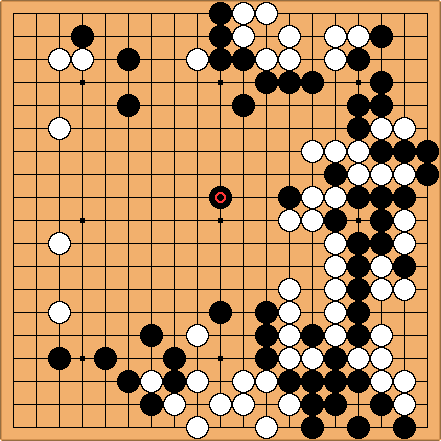
\includegraphics[height=0.6\paperheight]{game-board.png}
    \end{column}
    \end{columns}

    % Го -- стародавня стратегічна гра на двох гравців. Якщо розглядати її з боку теорії ігор, то вона є антагоністичною грою з повною інформацією.

    % Досі не було написано програму, що добре грає в Го. Основні труднощі...

    % Якщо говорити про розроблені програми, то більшість комерційна. Інші -- занадто складні.
\end{frame}

% III
\begin{frame}
    \frametitle{Існуючі рішення та їх недоліки}
    \begin{columns}
    \begin{column}{0.5\textwidth}
        \begin{itemize}
            \item CrazyStone -- комерційна;
            \item The Many Faces of Go -- комерційна;
            \item MoGo -- закрита;
            \item GNU Go -- неактуальна;
            \item Fuego -- заскладна;
            \item MasterGo -- комерційна;
            \item Kombilo -- немодульна.
        \end{itemize}
    \end{column}
    \begin{column}{0.5\textwidth}
        \hfill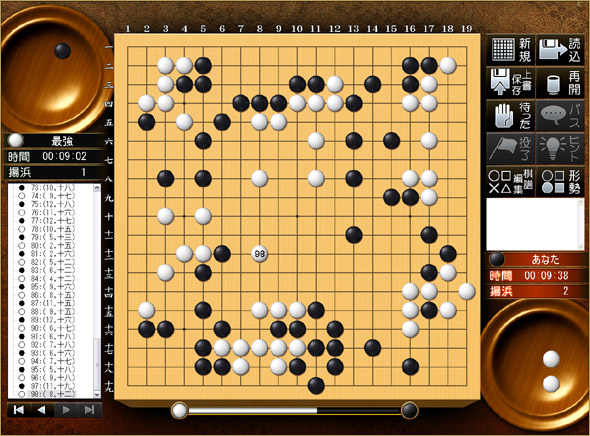
\includegraphics[height=0.4\paperheight]{crazystone.jpg}
    \end{column}
    \end{columns}

    % Комерційні програми не можуть бути використані ентузіастами для подальшого розвитку цієї галузі.

    % Некомерційні продукти -- складні, тобто вони мають багато різних модулів, котрі можуть взаємодіяти тільки між собою.
\end{frame}

% IV
\begin{frame}
    \frametitle{Мета проекту}
    Метою проекту є створення відкритої модульної системи для роботи зі структурами даних гри Го та надання користувачу функіоналу для паралельного пошуку партій та шаблонів у цих структурах.
    % Для роботи з SGF-файлами, перетворення їх у дерево варіантів гри. Також система повинна реалізовувати протокол GTP, для комунікації з іншими програмами.
\end{frame}

% V
\begin{frame}
    \frametitle{Основні задачі системи}
    \begin{itemize}
        \item Читання SGF-файлів, перетворення їх у внутрішнє дерево;
        \item пошук у цьому дереві методами
        \begin{itemize}
            \item Мінімакс;
            \item пошук за шаблоном;
            \item Монте-Карло.
        \end{itemize}
        % \item результуючий вивід, через протокол GTP.
    \end{itemize}
\end{frame}

% VI
\begin{frame}
    \frametitle{Структура системи пошуку}
    \center{
        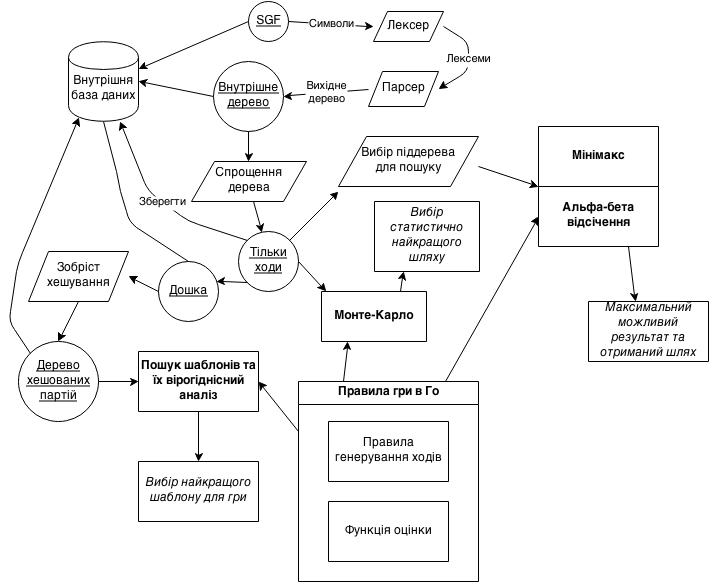
\includegraphics[height=0.8\paperheight]{structure_scheme.png}
    }

    % Жирним виділені самі алгоритми пошуку
    % Підкреслені - структури даних
    % Курсивом написані результуючі дані
\end{frame}


% VII
\begin{frame}
    \frametitle{Місце системи пошуку у системі, що грає в Го}
    \center{
        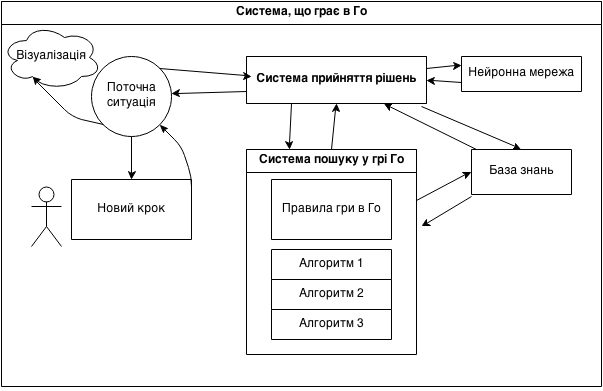
\includegraphics[width=0.8\paperwidth]{search_in_go_program.png}
    }

    % Усі алгоритми працюють однаково. Вони отримують потрібні їм структури даних (дерева або хешовані дошки) та правила гри в Го (правила генерування можливих ходів по поточному стану дошки та функція оцінки поточного стану дошки). Результат їх роботи -- наступний хід, що повинен зробити комп'ютер.

    % Саме тому їх можна використовувати у вигляді окремих модулів. Наприклад, як модулі інтелектуальної системи, для гри в Го.
\end{frame}

% VIII
\begin{frame}[fragile]
    \frametitle{Мінімаксний алгоритм пошуку по деревах}
    \begin{columns}
    \begin{column}{0.6\textwidth}
        \begin{algorithm}[H]
            \algsetup{linenosize=\tiny}

            \begin{algorithmic}[1]
                \REQUIRE Tree: node, Integer: depth
                \ENSURE Integer: value of best play
                    \IF {node is a terminal node \OR depth $\leq$ 0}
                        \RETURN the heuristic value of node
                    \ENDIF
                    \STATE $\alpha\gets-\infty$
                    \FORALL {childs of node}
                        \STATE $\alpha\gets$max($\alpha$, -minimax(child, depth-1))
                    \ENDFOR
                    \RETURN $\alpha$
            \end{algorithmic}
        \end{algorithm}
    \end{column}
    \begin{column}{0.4\textwidth}
        \hfill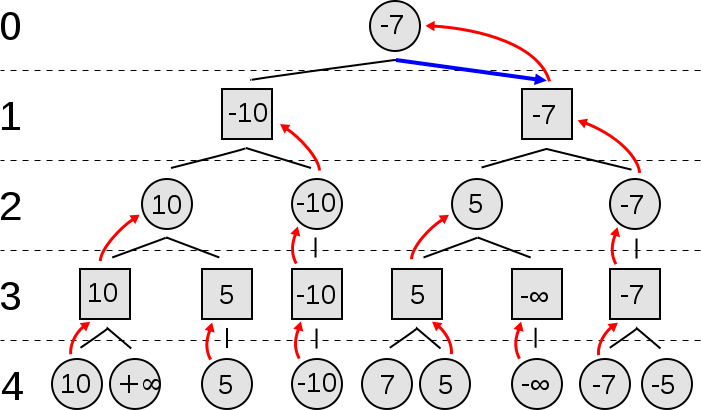
\includegraphics[height=0.3\paperheight]{minimax.png}
    \end{column}
    \end{columns}

    % Цей алгоритм використовує поняття мінімакса для пошуку оптимального шлягу при грі в Го. Він створює дерево гри, яке містить у собі всі можливі позиції на дошці. Далі, використовуючи функцію оцінки, він обирає шлях найбільш прийнятний на його ходах, та найменш прийнятний на ходах суперника. Алгоритм намагається максімізувати свій рахунок, у той час, як противник намагається мінімізувати його.

    % У цьому прикладі є можливість розпаралелити виконання алгоритму в точці пошуку максимального дочірнього вузла.
\end{frame}

% IX
\begin{frame}
    \frametitle{$\alpha-\beta$ відсічення}
    \begin{figure}
    \center{
        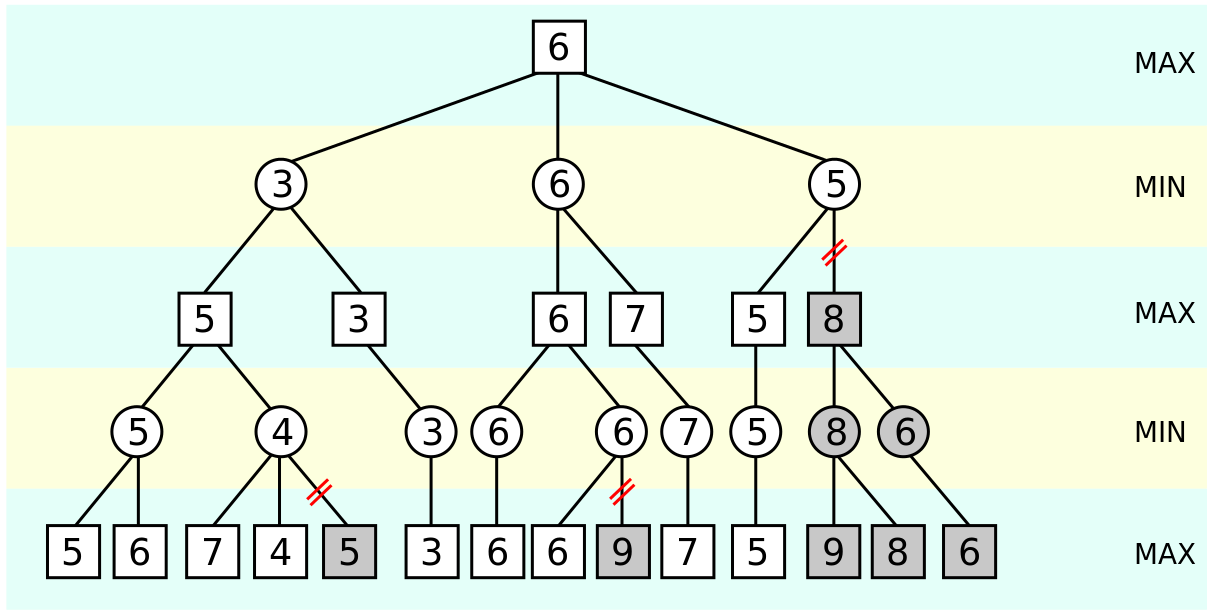
\includegraphics[width=0.8\paperwidth]{ab_pruning.png}
        \caption{Приклад роботи алгоритму}
    }\end{figure}

    % Це модифікація алгоритму мінімакса, що дає змогу відкидати деякі піддерева, що не є обов'язковими для обчислення. Ця оптимізація ніяк не впливає на результат алгоритму.
\end{frame}

% X
\begin{frame}
    \frametitle{Пошук по шаблонах}
    \begin{figure}
    \center{
        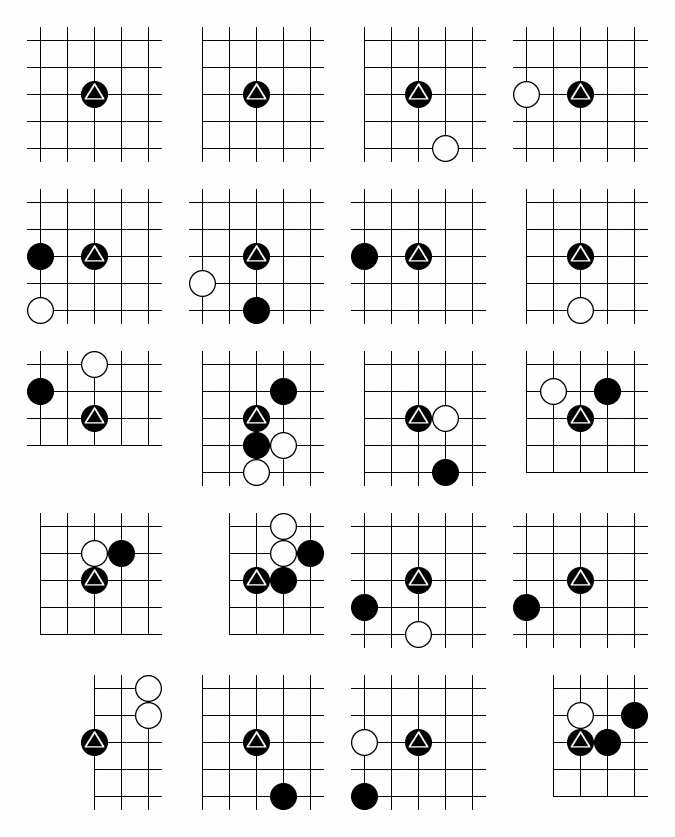
\includegraphics[height=0.6\paperheight]{patterns_frequency.png}
        \caption{20 найпопулярніших шаблонів у базі даних GnuGo}
    }\end{figure}
\end{frame}

% XI
\begin{frame}[fragile]
    \frametitle{Методи Монте-Карло}
    \begin{figure}
    \center{
        \includegraphics[height=1.0\paperheight]{monte-carlo_scheme.png}
        % \caption{Структурна схема методу Монте-Карло}
    }\end{figure}
    % \begin{lstlisting}
    % (defn play-game [board-state to-move]
    %     (if (terminal? board-state)                    ;return result
    %         (case to-move
    %             :black
    %             (let [mem (mcts-analyze-state board-state 30)   ;!1
    %                   move (mcts-select mem board-state)]          ;!2
    %                 (recur move (opp-player to-move)))
    %             :white
    %             (let [move (rand-nth (gen-children board-state))]
    %                 (recur move (opp-player to-move))))))
    % \end{lstlisting}
    % {
    %     \small
    %     \hspace*{\fill}Приклад коду, що грає в Го методом Монте-Карло\hspace*{\fill}
    % }

    % Метод імітації для приблизного відтворення реальних явищ. Він покладається на генерацію великої кількості випадкових величин, для отримання числового значення.
\end{frame}

% XII
\begin{frame}
    \frametitle{Метод верхньої оцінки значущості для дерев}
    \begin{equation*}
        UCTValue(parent,n)=winrate+\sqrt{\frac{\ln(parent.visits)}{5\times n.nodevisits}}
    \end{equation*}\\
    \bigskip
    Значущість вузла зменшується кожен раз, коли його відвідують. \\
    \medskip
    Але вона і збільшується кожен раз, коли батьківский вузол відвідують, але не обирають поточний вузол.
\end{frame}

% XIII
\begin{frame}
    \frametitle{Порівняння з існуючими продуктами}
    \begin{itemize}
        \item Проект відкритий, програмний код доступний на Github;
        \item система працює на платформі Java;
        \item система модульна, кожен модуль можна використовувати окремо.
    \end{itemize}
    \begin{figure}
    \center{
        
\includegraphics[height=0.4\paperheight]{github.png}
    }\end{figure}
\end{frame}

\begin{frame}
    \frametitle{Приклад роботи системи}
    \begin{figure}
    \center{
        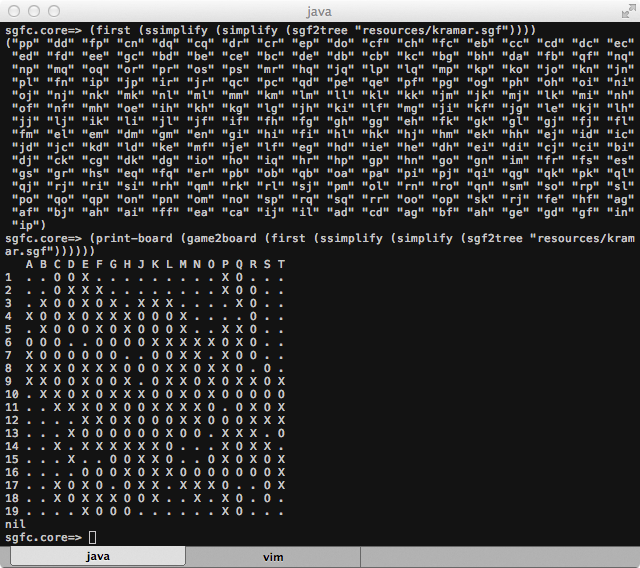
\includegraphics[height=0.7\paperheight]{screenshot.png}
        \caption{Приклад роботи з SGF-файлами}
    }\end{figure}
\end{frame}

\begin{frame}
    \frametitle{Розвиток системи}
    Для подальшого розвитку системи можна додати такий функціонал:
    \begin{itemize}
        \item Більше методів для пошуку у структурах даних
        \item Підтримку протоколу GTP, для спрощення комунікації з іншими модулями`'
    \end{itemize}
\end{frame}

% XV
\begin{frame}
    \frametitle{Висновки}
    В результаті дипломного проектування була створена система, що дозволяє користувачу:
    \begin{itemize}
        \item Працювати з SGF-файлами
        \item Спрощувати їх у внутрішню деревовидну структуру
        \item Використовувати методи Мінімакс, Монте-Карло та пошук за шаблоном
    \end{itemize}
\end{frame}

% XVI
\begin{frame}
    \frametitle{}
    \hspace*{\fill}\huge{Дякую за увагу!}\hspace*{\fill}
\end{frame}

\end{document}
